%\documentclass[a4paper]{scrartcl}
\documentclass[a4paper]{article}
\usepackage{fullpage}
\usepackage{url}
\usepackage{mdwlist}
\usepackage{polski}
\usepackage[utf8x]{inputenc}
\usepackage{color}
\usepackage{mathtools}
\usepackage{graphicx}
\usepackage[unicode=true]{hyperref}
\usepackage{multirow}
\usepackage[table]{xcolor}
\usepackage{listings}

\lstset{ %
basicstyle=\footnotesize,       % the size of the fonts that are used for the code
numbers=left,                   % where to put the line\dywiz numbers
numberstyle=\footnotesize,      % the size of the fonts that are used for the line\dywiz numbers
stepnumber=2,                   % the step between two line\dywiz numbers. If it's 1, each line 
% will be numbered
numbersep=5pt,                  % how far the line\dywiz numbers are from the code
frame=single,                   % adds a~frame around the code
}

\begin{document}
\sloppy

\title{coffeecam}
%\subtitle{silniczek graficzny w~coffeescripcie -- wirtualna kamera}
\author{Bartosz Pieńkowski, Barnaba Turek}
\maketitle
\abstract{
Celem serii projektów z~przedmiotu Grafika Komputerowa jest utworzenie prostego silnika graficznego 
(i~zapoznanie się od strony graficznej z~podstawowymi zadaniami grafiki komputerowej, takimi jak rzutowanie,
eliminacja elementów zasłoniętych i~cieniowanie). 

Zdecydowaliśmy się zaimplementować projekt w~języku coffeescript.

Pierwsza część projektu polega na utworzeniu wirtualnej kamery. Kamera ma obsługiwać zmianę pozycji, ogniskowej i~kąta, w~którym jest skierowana.
\begin{figure}[p!]
  \caption{Struktura projektu}
  \centering
  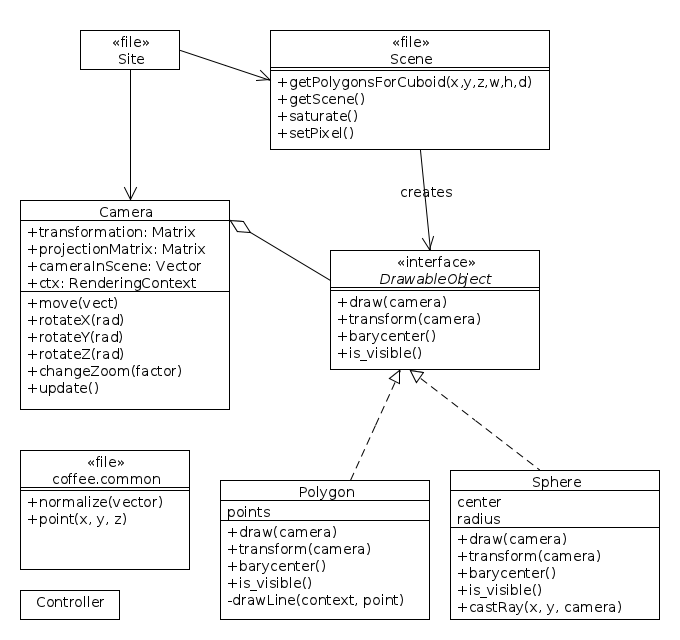
\includegraphics[width=\textwidth]{coffeecam_uml.png}
  \label{uml}
\end{figure}

\section{Wirtualna kamera}
\subsection{Struktura projektu}

Projekt podzielony jest na pliki .coffee, z~których każdy zostaje skomplikowany do pliku .js (javascript).
Zawartość każdego pliku wynikowego jest opakowana w~anonimową funkcję, aby zniwelować ryzyko konfliktu nazw z~innymi skryptami.

Zmienne i~funkcje potrzebne do komunikacji pomiędzy modułami dostępne są za pomocą zmiennej coffecam.

Nie wszystkie obiekty przedstawione na diagramie \ref{uml} są w~istocie klasami - z~wyjątkiem klas \textbf{Camera} i~\textbf{Controller}
nie potrzebowaliśmy przechowywać żadnego stanu, a~tylko logicznie podzielić udostępniane funkcje.

Plik \emph{site} jest swojego rodzaju funkcją main, która uruchamia się po załadowaniu dokumentu przez przeglądarkę.


\subsection{Działanie kamery}
Obiekt kamery przechowuje macierz transformacji, początkowo ustawioną na macierz jednostkową (z~dokładnością do znaku, ze względu na skrętności układów)\cite{openGL}.
Macierz transformacji obliczana jest na nowo po każdym ruchu kamery. Obliczenie nowej macierzy polega na pomnożeniu aktualnej macierzy przez żądaną transformacje.

Dostępne transformacje to przesunięcia i~obroty kamery (Transformacje utworzylismy na podstawie wykładu\cite{dasa}).

Po transformacji macierz transformacji mnożona jest przez macierz rzutowania (Obliczaną kiedy kamera jest tworzona i~przy zmianie ogniskowej)\cite{openGL}.
Następnie każdy z~punktów sceny mnożony jest przez macierz wynikową.
Przygotowanie każdej nowej klatki realizuje metoda \emph{update()} kamery.

\subsection{Scena}
Obiekty, które kamera wyświetla to wielokąty.
Kamera zakłada, że punkty obiektu podane są w~sposób uporządkowany.

Scena tworzona jest z~czworokątów, ze względu na to, że rysujemy głównie prostopadłościany.
\newpage
\subsection{Pozostałe informacje o~projekcie}
Statyczne części projektu (strony, style) są tworzone za pomocą frameworku \href{http://staticmatic.rubyforge.org/}{staticmatic}, na podstawie źródeł (W~językach \href{http://haml-lang.com/}{HAML} i~\href{http://sass-lang.com/}{SASS}).

W~projekcie wykorzystaliśmy javascriptową bibliotekę \href{http://sylvester.jcoglan.com/}{Sylvester} wspierającą operacje na macierzach i~wektorach.

Kod źródłowy projektu (wraz z~aktualną dokumentacją) dostępny jest na serwisie \href{https://github.com/barnaba/coffeecam}{Github} (głównie katalog /src/coffee).

Projekt jest dostępny do testowania na następujących serwerach:
\begin{itemize}
  \item \href{http://barnex.mooo.com/}{Serwer 1}\footnote{\url{http://barnex.mooo.com}}
  \item \href{http://volt.iem.pw.edu.pl/~pienkowb/}{Volt}\footnote{\url{http://volt.iem.pw.edu.pl/~pienkowb/}} (Niekoniecznie aktualna wersja)
\end{itemize}

\begin{thebibliography}{9}

\bibitem{openGL}
  Song Ho Ahn,
  OpenGL Projection Matrix,
  \url{http://www.songho.ca/opengl/gl_projectionmatrix.html}

\bibitem{dasa}
  Dariusz Sawicki,
  Grafika komputerowa i~wizualizacja,
  \url{http://wazniak.mimuw.edu.pl/index.php?title=Grafika_komputerowa_i_wizualizacja}

\end{thebibliography}

\end{document}

